
\subsection{Classical correlation set}\label{sec:classical-correlation-set}

\begin{defn}\label{defn:classical-correlation-set}
    The set $C_{c}(n, k)$ of \emph{classical correlations} is the set of tuples $\left(p_{a b x y}\right)$ such that there exists a set $\Lambda$ with probability measure $v$ and for every $\lambda \in \Lambda$ functions $A^{\lambda}, B^{\lambda}:\{1,2, \ldots, n\} \rightarrow\{1,2, \ldots, k\}$ such that
    \begin{equation}
        \begin{split}
    &\forall x, y \in\{1,2, \ldots, n\}, \quad \forall a, b \in\{1,2, \ldots, k\}, \\
     &p_{a b x y}  =\operatorname{Pr}_{\lambda \sim v}\left(A^{\lambda}(x)=a \wedge B^{\lambda}(y)=b\right) .
        \end{split}
    \end{equation}

    Of course $C_{c}(n, k) \subseteq [0,1]^{n^2k^2}$~\cite{mipre}.
\end{defn}


\begin{figure}[htb]
    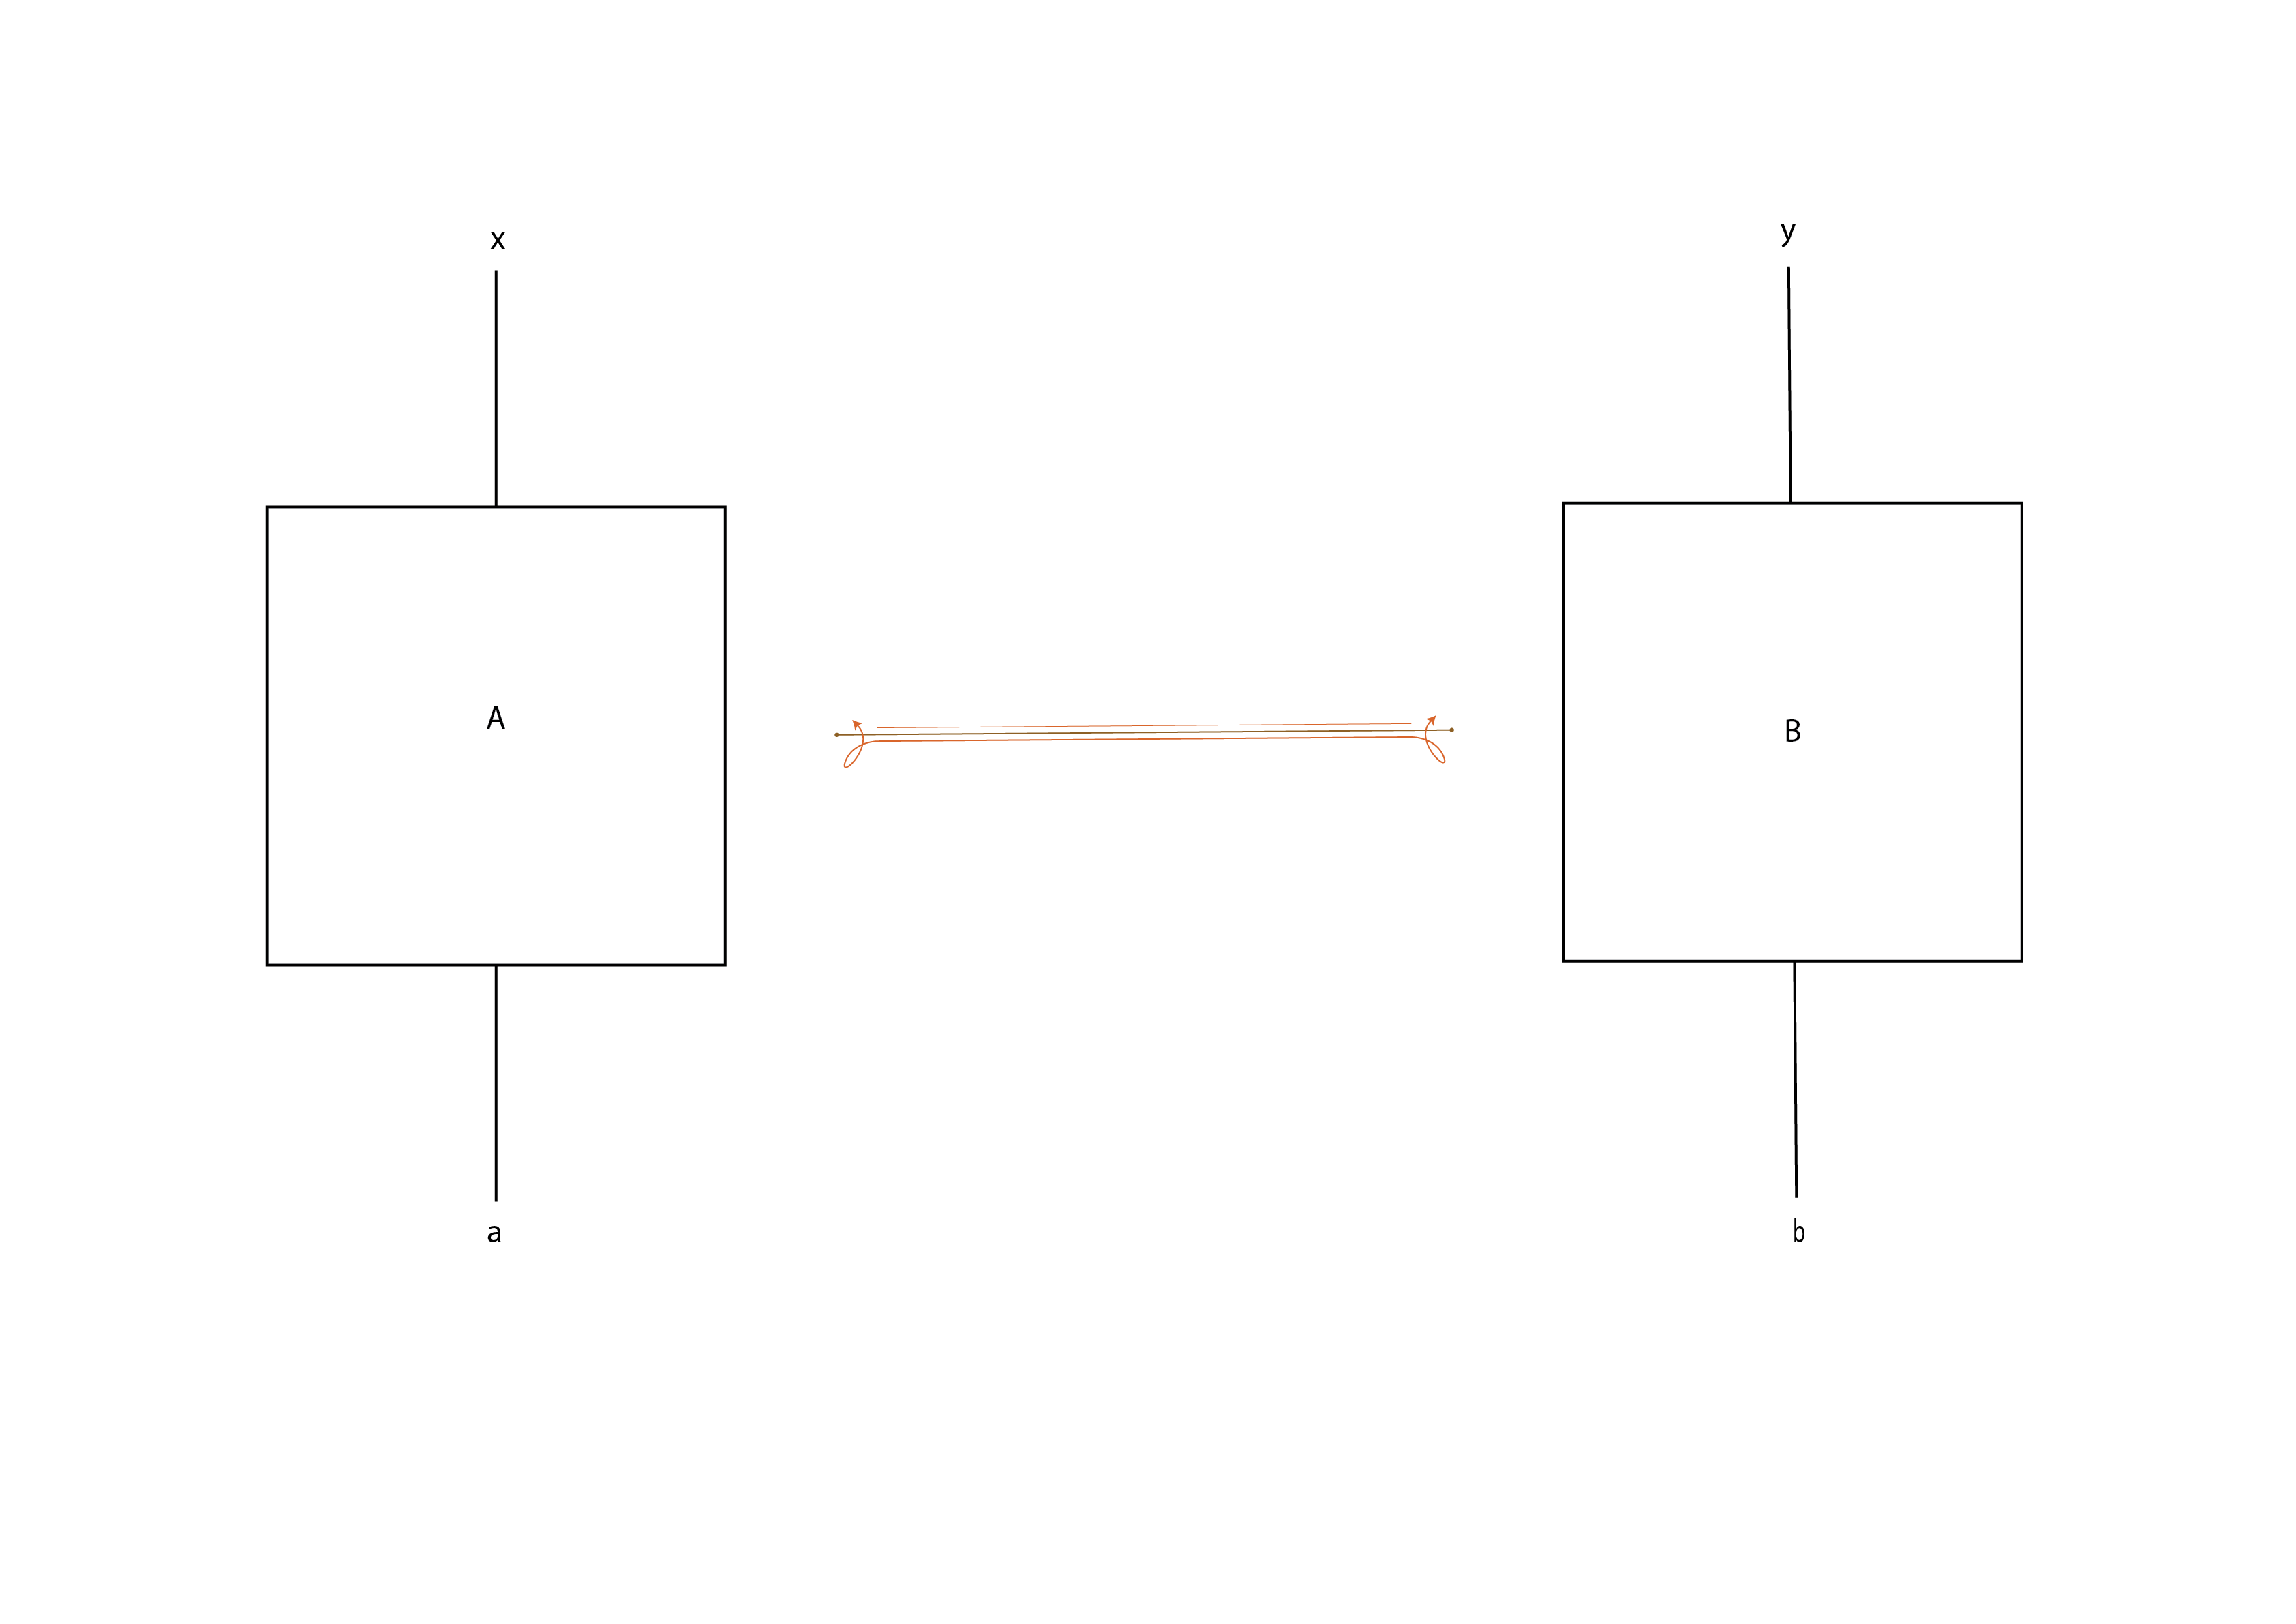
\includegraphics[width=\linewidth]{Correlations.png}
    \centering
    \caption{Visual representation of correlations.}
    \end{figure}